\documentclass[12pt]{report}

% packages used for many things
\usepackage[utf8]{inputenc}
\usepackage[english]{babel}
\usepackage{hyperref}
\hypersetup{
    colorlinks=true,
    linkcolor=blue,
    filecolor=magenta,      
    urlcolor=cyan,
}
\urlstyle{same}
\usepackage{enumitem}
\usepackage{amsmath}
\usepackage{mathtools}
\usepackage{amsfonts} 
\usepackage{amssymb}
\usepackage{MnSymbol}
\usepackage{csquotes}
\usepackage{arydshln}
\usepackage{algorithm}
\usepackage{algorithmic}
\usepackage{extarrows}
\usepackage{tikz}
\usepackage{comment}

% declare here the expectation symbol
\DeclareMathOperator{\E}{\mathbb{E}}

% argmin operator
\DeclareMathOperator*{\argmin}{\arg\!\min}

% for text over equal sign
\newcommand\prone{\mathrel{\overset{\makebox[0pt]
    {\mbox{\normalfont\tiny\sffamily (1)}}}{=}}}
\newcommand\prtwo{\mathrel{\overset{\makebox[0pt]
    {\mbox{\normalfont\tiny\sffamily (2)}}}{=}}}
\newcommand\prthr{\mathrel{\overset{\makebox[0pt]
    {\mbox{\normalfont\tiny\sffamily (3)}}}{=}}}


% for images
\usepackage{graphicx}
\graphicspath{{./images/}}

% qed black square
\newcommand*{\QEDA}{\hfill\ensuremath{\blacksquare}}


% Author of this mathematical analysis
\begin{comment}
    @ Author: Andreas Spanopoulos
\end{comment}

% title, date, etc..
\title{Variational Autoencoder Mathematics}
\author{\LARGE{Andreas Spanopoulos} \\ andrewspanopoulos@gmail.com}


% ----------------    START OF DOCUMENT    ------------ %
\begin{document}
\maketitle

% --------------------           PAGE 1           ---------------------- %
\section*{Introduction}
\smallskip

The \textbf{Variational Autoencoder} (aka \textbf{VAE}) is a generative model.
This means that it is a model which produces new unseen data. Unlike the normal
Autoencoder, VAE focuses on understanding the distribution of a smaller
representation of the data. This lower-dimensional representation of the data is
known as \textquote{latent vector $\textbf{z}$}.
\bigskip

The dimension of the latent vector z is a hyperparameter which we choose along
with the architecture of the Network. Keep in mind that we don't want
$\textbf{z}$ to be too large. It should be a relatively small vector, so that an
information bottleneck is created. One other reason for $\textbf{z}$ being small,
is that we want to be able to sample easily new vectors, without having to take
into consideration many features.
\bigskip

With that said, the question arises: How can we pick the values of $\textbf{z}$
which will make sense, that is, which will generate a new data point from the
distribution of our original data?
\bigskip

Here is the beauty of the \textbf{Variational Autoencoder}: We will learn the
distribution of $\textbf{z}$. That is, for every component of $\textbf{z}$, we
will learn a mean and a standard deviation.
\bigskip

Suppose $\textbf{z}$ has $k$ components:
\begin{align*}
    z \;=\;
    \begin{bmatrix}
        z_1 \\
        z_2 \\
        \vdots \\
        z_k
    \end{bmatrix}
\end{align*}
Then, the mean and standard deviation vectors are defined as:
\begin{align*}
    \mu \;=\;
    \begin{bmatrix}
        \mu_1 \\
        \mu_2 \\
        \vdots \\
        \mu_k
    \end{bmatrix}
    ,\quad \sigma \;=\;
    \begin{bmatrix}
        \sigma_1 \\
        \sigma_2 \\
        \vdots \\
        \sigma_k
    \end{bmatrix}
\end{align*}
Our goal is to learn the $\mu$ and $\sigma$ vectors in order to be able to sample
$\textbf{z}$ as follows $$z \;=\; \mu + \epsilon \odot \sigma$$
where $\epsilon \sim N(0, 1)$ is a gaussian with mean 0 and standard deviation 1.
\clearpage

% --------------------           PAGE 2           ---------------------- %
\begin{figure}
    \includegraphics[scale=0.31]{vae-gaussian.png}   
    \caption{This picture demonstrates the architecture of a Variational
             Autoencoder. The input \textbf{x} gets fed in a Probabilistic
             Encoder $q_{\phi}(z | x)$, which in turns connects with the
             $\mu$ and $\sigma$ layers. Note that usually there is a encoder
             Network before the mean and std layers, but here in the figure
             it is ommitted. Then, they sample $\textbf{z}$ which
             in turn is fed to the Probabilistic Decoder $p_{\theta}(x | z)$.
             The result is then fed to an output layer which represents the
             reconstructed input data. The original picture can be found
             \href{https://blog.bayeslabs.co/2019/06/04/All-you-need-to-
             know-about-Vae.html}{here}.}
    \label{fig:Architecture}
\end{figure}

\subsection*{Brief Explanation of architecture}
The architecture of a \textbf{VAE} is briefly portrayed in 
Figure~\ref{fig:Architecture}. Let's take a closer look in each part:

\begin{enumerate}
    \item The encoder part consists of a Probabilistic Encoder $q_{\phi}(z | x)$.
        Given some parameters $\phi$ (which are parameters of the model),
        $q_{\phi}(z | x)$ models the probability of obtaining the latent vector
        $\textbf{z}$ given input data $\textbf{x}$. Afterwards, it connects to
        the $\mu$ and $\sigma$ layers, as there might a whole encoder network
        before those.
    \item The latent vector $\textbf{z}$.
    \item The decoder part which consists of a Probabilistic Decoder
        $p_{\theta}(x | z)$. As with the probabilistic encoder, given some
        parameters $\theta$ which are parameters of the model, we want to learn
        the probability of obtaining a data point $\textbf{x}$ given a latent
        vector $\textbf{z}$.
    \item The reconstructed input $\hat{x}$.
\end{enumerate}
\clearpage

% --------------------           PAGE 3           ---------------------- %
\section*{Loss function}
The loss function of the VAE is:
\begin{align*}
    L(\theta,\, \phi,\, x) \;=\; -\E_{z \sim q_{\phi}(z | x)}
                                    \left[\log p_{\theta}(x | z) \right]\;
                              +\; D_{KL}\left[q_{\phi}(z | x) \;||\; p_{\theta}(z) \right]
\end{align*}
It may seem daunting at first, but if we break it down into pieces then it gets
much simpler.

\subsection*{KL-Divergence and multivariate Normal Distribution}
Let's start by explaining what the second term of the loss function is. The
\textbf{K}ullback \textbf{L}eibler Divergence, also known as
\href{https://en.wikipedia.org/wiki/Relative_entropy}{Relative Entropy}, is
a measure of similarity between two probability distributions. It is denoted by
$D_{KL}(\cdot \;||\; \cdot)$, its unit of measure it called \textbf{nat} and it
can computed by the formula (for continuous probability distributions $P,\; Q$):
\begin{equation}\label{eq:KLD}
    D_{KL} \left[ P \,||\, Q \right] \;=\;
        \int P(x) \log\left(\frac{P(x)}{Q(x)}\right) dx
\end{equation}
Of course, this implies that $D_{KL} (P \,||\, Q) \neq D_{KL} (Q \,||\, P)$.
\bigskip

Now, let's suppose that both $P,\; Q$ are multivariate
normal distributions with means $\mu_1, \mu_2$ and
\href{https://en.wikipedia.org/wiki/Covariance_matrix}{covariance} matrices
$\Sigma_1, \Sigma_2$:
\begin{align*}
P(x) \,=&\, N(x;\, \mu_1,\, \Sigma_1) \,=\,
    \frac{1}{\sqrt{(2\pi)^k|\Sigma_1|}}
    e^{-\frac{1}{2}(x-\mu_1)^T\Sigma_1^{-1}(x - \mu_1)} \\
Q(x) \,=&\, N(x;\, \mu_2,\, \Sigma_2) \,=\,
    \frac{1}{\sqrt{(2\pi)^k|\Sigma_2|}}
    e^{-\frac{1}{2}(x-\mu_2)^T\Sigma_2^{-1}(x - \mu_2)}
\end{align*}
where $k$ is the magnitude (length) of vector $x$.
\smallskip

\noindent Hence
\begin{align*}
    \log(P(x)) \;=\;& \log\left(\frac{1}{\sqrt{(2\pi)^k|\Sigma_1|}}
                e^{-\frac{1}{2}(x-\mu_1)^T\Sigma_1^{-1}(x - \mu_1)} \right) \\
               \;=\;& \log \left( \frac{1}{\sqrt{(2\pi)^k|\Sigma_1|}} \right) +
                \log \left( e^{-\frac{1}{2}(x-\mu_1)^T\Sigma_1^{-1}
                (x - \mu_1)} \right) \\
               \;=\;& -\frac{k}{2}\log(2\pi) -\frac{1}{2}\log(|\Sigma_1|) -
                \frac{1}{2}(x-\mu_1)^T\Sigma_1^{-1} (x - \mu_1)
\end{align*}
\clearpage

% --------------------           PAGE 4           ---------------------- %
\noindent Following the exact same steps, we also get that
\begin{align*}
    \log(Q(x)) \;=\; -\frac{k}{2}\log(2\pi) -\frac{1}{2}\log(|\Sigma_2|) -
    \frac{1}{2}(x-\mu_2)^T\Sigma_2^{-1} (x - \mu_2)
\end{align*}

\noindent With the help of the above equalities, expanding \eqref{eq:KLD} yields:

\begin{align*}
    D_{KL} \left[ P \,||\, Q \right]
    \;=&\; \int P(x) \left[\log(P(x)) - \log(Q(x)) \right] dx\\
    \;=&\; \int P(x) \left[ \frac{1}{2}\log\left(\frac{|\Sigma_2|}{|\Sigma_1|}\right)
        - \frac{1}{2}(x-\mu_1)^T\Sigma_1^{-1} (x - \mu_1) \right. \\
       &\left.\qquad\qquad\qquad\qquad\quad\;\;\;\,
        + \frac{1}{2}(x-\mu_2)^T\Sigma_2^{-1} (x - \mu_2)\right] dx
\end{align*}
We can rewrite the above term an an Expectation over $P$:
\begin{align*}
    D_{KL} \left[ P \,||\, Q \right]
    \;=&\; \E_P \left[ \frac{1}{2}\log\left(\frac{|\Sigma_2|}{|\Sigma_1|}\right)
        - \frac{1}{2}(x-\mu_1)^T\Sigma_1^{-1} (x - \mu_1) \right. \\
       &\left.\qquad\qquad\qquad\quad\;\;\,
        + \frac{1}{2}(x-\mu_2)^T\Sigma_2^{-1} (x - \mu_2)\right]
\end{align*}
Since the logarithmic term is independent of $x$, we can move it outside the
expectation. This leaves us with
\begin{align}\label{eq:kld_exp}
    D_{KL} \left[ P \,||\, Q \right]
    \;=\quad &\frac{1}{2}\log\left(\frac{|\Sigma_2|}{|\Sigma_1|}\right) \nonumber \\
       \; -\, &\frac{1}{2} \E_P \left[ (x-\mu_1)^T\Sigma_1^{-1} (x - \mu_1) \right]
            \nonumber \\
       \; +\, &\frac{1}{2} \E_P \left[ (x-\mu_2)^T\Sigma_2^{-1} (x - \mu_2) \right]
\end{align}
Let's now try to simplify the 2nd and 3rd terms of the above expression.
\bigskip

\noindent First, we have to recall the
\href{https://en.wikipedia.org/wiki/Trace_(linear_algebra)}{trace}
function and some of its properties. The trace of a square matrix $A$,
denoted as $tr(A)$, is the sum of the elements along the main diagonal of $A$.
The \href{https://en.wikipedia.org/wiki/Trace_(linear_algebra)#Properties}{properties}
of the trace function which we will need are:
\begin{enumerate}
    \item \href{https://math.stackexchange.com/questions/3098841/how-could-a-scalar-
        be-equal-to-the-trace-of-the-same-scalar}{Trace of scalar}:
        Considering the scalar as a $1\times1$ matrix, gives: $x = tr(x)$
    \item \href{https://math.stackexchange.com/questions/2228398/trace-trick-for-
        expectations-of-quadratic-forms}{Trace of Expectation}:
        From 1: $\E[x] = \E[tr(x)] \Rightarrow tr(\E[x]) = \E[tr(x)]$
    \item \href{https://en.wikipedia.org/wiki/Trace_(linear_algebra)#Cyclic_property}
        {Cyclic Property}: $tr(ABC) \;=\; tr(CAB)$
\end{enumerate}
\clearpage

% --------------------           PAGE 5            ---------------------- %
\noindent Having these properties in mind, we are now ready to simplify the
expectation terms computed before during the simplification of the KL Divergence.

\begin{itemize}
    \item Term 2. Note that the matrix multiplications inside the expectation reduce
        to a scalar value.
        \begin{align*}
            \E_P \left[ (x-\mu_1)^T\Sigma_1^{-1} (x - \mu_1) \right]
            \;\prone\;& \E_P \left[ tr\left((x-\mu_1)^T\Sigma_1^{-1}
                (x - \mu_1)\right) \right] \\
            \;\prthr\;& \E_P \left[ tr\left( (x - \mu_1)(x - \mu_1)^T
                \Sigma_1^{-1} \right) \right] \\
            \;\prtwo\;& tr\left( \E_P\left[ (x - \mu_1)(x - \mu_1)^T
                \Sigma_1^{-1} \right] \right)
        \end{align*}
        $\Sigma_1^{-1}$ is independent from the expectation over $P$, so it can
        be moved outside, thus giving:
        \begin{align*}
            \E_P \left[ (x-\mu_1)^T\Sigma_1^{-1} (x - \mu_1) \right] \;=\;
                tr\left( \E_P\left[ (x - \mu_1)(x - \mu_1)^T
                    \right] \Sigma_1^{-1} \right)
        \end{align*}
        But the term $E_P\left[ (x - \mu_1)(x - \mu_1)^T \right]$ is equal to the
        \href{https://en.wikipedia.org/wiki/Covariance_matrix#Definition}
        {Covariance Matrix} $\Sigma_1$, thus yielding
        \begin{align}\label{eq:kld_term2}
            \E_P \left[ (x-\mu_1)^T\Sigma_1^{-1} (x - \mu_1) \right]
                \;=\; tr\left( \Sigma_1 \Sigma_1^{-1} \right) \;=\; tr(I_k) \;=\; k
        \end{align}
    \item Term 3. Again, the term inside the expectation reduces to a scalar.
        \begin{align*}
            \E_P &\left[ (x - \mu_2)^T\Sigma_2^{-1} (x - \mu_2) \right] \\[2ex]
            \mbox{Add and}& \mbox{ subtract } \mu_1: \\[2ex]
            \;=&\; \E_P \left[ [(x - \mu_1) + (\mu_1 - \mu_2)]^T\Sigma_2^{-1}
                [(x - \mu_1) + (\mu_1 - \mu_2)] \right] \\[2ex]
            \;=&\; \E_P \left[ \left[(x - \mu_1)^T + (\mu_1 - \mu_2)^T\right]
                \Sigma_2^{-1} [(x - \mu_1) + (\mu_1 - \mu_2)] \right] \\[2.5ex]
            (A^T + B^T&)C(A + B) \;=\; A^TCA + A^TCB + B^TCA + B^TB: \\[2.5ex]
            \;=&\; \E_P \left[ (x - \mu_1)^T\Sigma_2^{-1}(x - \mu_1) \;+\;
                (x - \mu_1)^T\Sigma_2^{-1}(\mu_1 - \mu_2) \;+ \right. \\[2ex]
                & \quad\;\;\;\,
                \left. (\mu_1 - \mu_2)^T\Sigma_2^{-1}(x - \mu_1) \;+\; 
                (\mu_1 - \mu_2)^T\Sigma_2^{-1}(\mu_1 - \mu_2) \right]
        \end{align*}
        \clearpage
% --------------------           PAGE 6            ---------------------- %
        Taking the expectation over each term individually:
        \begin{align*}
            \E_P \left[(x - \mu_2)^T\Sigma_2^{-1} (x - \mu_2)\right]
            \;=\; &\E_P \left[(x - \mu_1)^T\Sigma_2^{-1}(x - \mu_1)\right] \;+\\[2ex]
                  &\E_P \left[(x - \mu_1)^T\Sigma_2^{-1}(\mu_1 - \mu_2)\right]\;+\\[2ex]
                  &\E_P \left[(\mu_1 - \mu_2)^T\Sigma_2^{-1}(x - \mu_1)\right]\;+\\[2ex]
                  &\E_P \left[(\mu_1 - \mu_2)^T\Sigma_2^{-1}(\mu_1 - \mu_2)\right]
        \end{align*}
        \begin{itemize}
            \item The first sub-term has the same derivation as the first
                term from before:
                $$\E_P \left[ (x - \mu_1)^T\Sigma_2^{-1}(x - \mu_1) \right] \;=\;
                    tr(\Sigma_1\Sigma_2^{-1})$$
            \item The second and third sub-terms are equal to $0$ due to the
                expectation over $(x - \mu_1)^T$. Specifically, the factor
                $\Sigma_2^{-1} (\mu_1 - \mu_2)$ can be moved out of the expectation
                as it is a constant:
                \begin{align*}
                    \E_P \left[ (x - \mu_1)^T\Sigma_2^{-1}(\mu_1 - \mu_2) \right]
                    \;=&\; \E_P \left[ (x - \mu_1)^T \right]
                        \Sigma_2^{-1}(\mu_1 - \mu_2) \\
                    \;=&\; 0_k \; \Sigma_2^{-1}(\mu_1 - \mu_2) \;=\; 0 \\[1.5ex]
                    \E_P \left[ (\mu_1 - \mu_2)^T\Sigma_2^{-1}(x - \mu_1) \right]
                    \;=&\; (\mu_1 - \mu_2)^T\Sigma_2^{-1}
                        \E_P \left[ (x - \mu_1)^T \right] \\
                    \;=&\; \Sigma_2^{-1}(\mu_1 - \mu_2) \; 0_k \;=\; 0
                \end{align*}
            \item The fourth sub-term is the expectation of a constant, so it is equal
                to the constant itself:
                $$\E_P \left[ (\mu_1 - \mu_2)^T\Sigma_2^{-1}(\mu_1 - \mu_2)\right] \;=\;
                (\mu_1 - \mu_2)^T\Sigma_2^{-1}(\mu_1 - \mu_2)$$
        \end{itemize}
    These simplifications leave us with:
    \begin{align}\label{eq:kld_term3}
        \E_P \left[ (x - \mu_2)^T\Sigma_2^{-1} (x - \mu_2) \right] \;=\;\,
        &tr(\Sigma_1\Sigma_2^{-1}) \,+ \nonumber \\
        &(\mu_1 - \mu_2)^T\Sigma_2^{-1}(\mu_1 - \mu_2)
    \end{align}
\end{itemize}

\noindent Finally, formula \eqref{eq:kld_exp} for the KL-Divergence can be ultimately
simplified using equations \eqref{eq:kld_term2}, \eqref{eq:kld_term3} to:
\begin{align}\label{eq:kld_gauss}
    D_{KL} \left[ P \,||\, Q \right] \;=\;
    \frac{1}{2}\left[ \log\left(\frac{|\Sigma_2|}{|\Sigma_1|}\right) \;-\;
    k \;+\;
    tr(\Sigma_1\Sigma_2^{-1}) \;+\; (\mu_1 - \mu_2)^T\Sigma_2^{-1}
        (\mu_1 - \mu_2) \right]
\end{align}
\QEDA
\clearpage

% --------------------           PAGE 7            ---------------------- %
\subsection*{Goal of VAE}
As mentioned in the introduction, the goal of the \textbf{VAE} is to learn the
distribution $q_{\phi}(\textbf{z} | \textbf{x})$ of the latent vector $\textbf{z}$.
After the distribution of the latent vector has been learnt, we can sample
$\textbf{z}$ and feed it to the Generator Network defined by the distribution
$p_{\theta}(\textbf{x} | \textbf{z})$ (aka decoder) in order to obtain a new
data point $\tilde{x}$. Of course during training, we want $\tilde{x} \approx x$.
The training process can be thought of graphically as follows
\bigskip

\begin{center}
    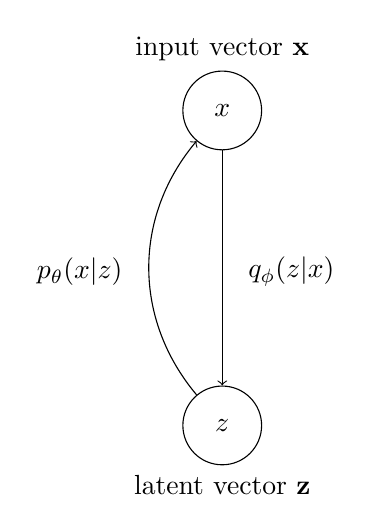
\begin{tikzpicture}
        % nodes x, z
        \node[draw, circle, minimum size=1cm, inner sep=0pt,
        label=above:input vector $\textbf{x}$] (x) at (0, 0) {$x$};
        \node[draw, circle, minimum size=1cm, inner sep=0pt,
            label=below:latent vector $\textbf{z}$] (z) at (0, -4) {$z$};

        % edge q_phi
        \draw[->] (x) to node[midway, above, xshift=25, yshift=-10]
            {$q_{\phi}(z | x)$} (z);
        % edge p_theta
        \draw[->] (z) to[bend right=-40] node[midway, above, xshift=-25, yshift=-10]
            {$p_{\theta}(x | z)$} (x);
    \end{tikzpicture}
\end{center}
\bigskip

\subsection*{Derivation of Loss Function}
We would like the two distributions to be approximately same, that is
$$q_{\phi}(z | x) \approx p_{\theta}(z| x)$$
How can we force the two distributions to come close? We could view this
as a minimization problem of the KL-Divergence between $Q$ and $P$.
\begin{align*}
    D_{KL} \left[ q_{\phi}(z | x) \,||\, p_{\theta}(z | x) \right]
    \;=\; \int q_{\phi}(z | x) \log \left(
        \frac{q_{\phi}(z | x)}{p_{\theta}(z | x)} \right) dz
\end{align*}
\clearpage

% --------------------           PAGE 8            ---------------------- %
Rewriting this term as an Expectation yields:
\begin{align*}
    D_{KL} &\left[ q_{\phi}(z | x) \,||\, p_{\theta}(z | x) \right] \\[2ex]
    \;=&\; \E_{z \sim q_{\phi}(z|x)}\left[ \log \left(
        \frac{q_{\phi}(z | x)}{p_{\theta}(z | x)} \right) \right] \\[2ex]
    \;=&\; \E_{z \sim q_{\phi}(z|x)}\left[ \log q_{\phi}(z | x)
        - \log p_{\theta}(z | x) \right] \\[2ex]
    \;=&\; \E_{z \sim q_{\phi}(z|x)}\left[ \log q_{\phi}(z | x)
        - \log \left( \frac{p_{\theta}(x | z) \; p_{\theta}(z)}
            {p_{\theta}(x)} \right) \right] \\[2ex]
    \;=&\; \E_{z \sim q_{\phi}(z|x)}\left[ \log q_{\phi}(z | x)
        - \log p_{\theta}(x | z) - \log p_{\theta}(z)
            + \log p_{\theta}(x) \right]
    % \;=&\; \E_{z \sim q_{\phi}(z|x)} [\log q_{\phi}(z | x)] -
    %        \E_{z \sim q_{\phi}(z|x)} [\log p_{\theta}(x | z)] \,-\\[2ex]
    %    &\; \E_{z \sim q_{\phi}(z|x)} [\log p_{\theta}(z)] +
    %        \E_{z \sim q_{\phi}(z|x)} [\log p_{\theta}(x)] 
\end{align*}
Since $\log p_{\theta}(x)$ is independent from the Expectation of $z$, it can be moved
outside, thus giving
\begin{align*}
    D_{KL} &\left[ q_{\phi}(z | x) \,||\, p_{\theta}(z | x) \right]
        - \log p_{\theta}(x) \\[2ex]
    \;=&\; -\E_{z \sim q_{\phi}(z|x)}[\log p_{\theta}(x | z)] \;+\;
        \E_{z \sim q_{\phi}(z|x)}[\log q_{\phi}(z | x) - \log p_{\theta}(z)] \\[2ex]
    \;=&\; -\E_{z \sim q_{\phi}(z|x)}[\log p_{\theta}(x | z)] \;+\;
        \E_{z \sim q_{\phi}(z|x)} \left[ \log \left(
        \frac{q_{\phi}(z | x)}{p_{\theta}(z)} \right) \right] \\[2ex]
    \;=&\; -\E_{z \sim q_{\phi}(z|x)}[\log p_{\theta}(x | z)] \;+\;
        D_{KL} \left[ q_{\phi}(z | x) \,||\, p_{\theta}(z) \right]
\end{align*}
which is the loss function $L$, defined in terms of $\phi,\, \theta,\, x$:
\begin{align*}
    L(\theta,\, \phi,\, x) \;=\; -\E_{z \sim q_{\phi}(z | x)}
                                    \left[\log p_{\theta}(x | z) \right]\;
                              +\; D_{KL}\left[q_{\phi}(z | x) \;||\; p_{\theta}(z) \right]
\end{align*}
which is also known as
\href{https://en.wikipedia.org/wiki/Variational_Bayesian_methods#Evidence_lower_bound}
{Evidence Lower BOund} (ELBO).
Of course, our target is to find the $\theta,\, \phi$ that minimize the loss
$L(\theta,\, \phi,\, x)$ for all data points $x$ in the training set, $X$ that is:
$$\theta^*,\, \phi^* \;=\; \argmin_{\phi,\, \theta} L(\theta,\, \phi,\, x)
\text{ over all } x \in X$$
Where in our case $\theta^*$ are the weighs of the Recognition Network (aka encoder)
and $\phi^*$ are the weights of the Generator Network (aka decoder). \clearpage

% --------------------           PAGE 9            ---------------------- %
\subsection*{Simplifying the Loss Function}
How could we simplify the Loss function $L(\theta,\, \phi,\, x)$ such that it can be
computed using known information? The problem is the KL-Divergence term, as we don't
have a closed form for it. The first solution that comes to mind is to model both
distributions of the KL-Divergence term as Gaussians, with $p_{\theta}(z)$ having
mean 0 and standard deviation 1, thus pushing $q_{\phi}(z | x)$ to come close
to it. Specifically:
\begin{enumerate}
    \item $q_{\phi}(z | x) \sim N(\mu_{\phi}(x),\, \Sigma_{\phi}(x))$
    \item $p_{\theta}(z) \sim N(0_k,\, I_k)$
\end{enumerate}

\noindent This in turn allows us to use eq. \eqref{eq:kld_gauss}, substituting the values
\begin{enumerate}
    \item $\mu_1 \,=\, \mu_{\phi}(x),\; \Sigma_1 \,=\, \Sigma_{\phi}(x)$
    \item $\mu_2 \,=\, 0_k,\; \Sigma_2 \,=\, I_k$
\end{enumerate}
Thus yielding:
\begin{align*}
    D_{KL}&\left[q_{\phi}(z | x) \;||\; p_{\theta}(z) \right] \\[2ex]
    \;=&\; \frac{1}{2} \left[ \log \left(\frac{|I_k|}{|\Sigma_{\phi}(x)|} \right)
        - k
        + tr(\Sigma_{\phi}(x) \, I_k)
        + (\mu_{\phi}(x) - 0_k)^T I_k (\mu_{\phi}(x) - 0_k) \right] \\[2ex]
    \;=&\; \frac{1}{2} \left[ -\log |\Sigma_{\phi}(x)|
        - k
        + tr(\Sigma_{\phi}(x))
        + \mu_{\phi}(x)^T \mu_{\phi}(x) \right]
\end{align*}
Note that $\Sigma_{\phi}(x)$ is a diagonal matrix with $k$ elements. Hence we can
write
\begin{align*}
    D_{KL}&\left[q_{\phi}(z | x) \;||\; p_{\theta}(z) \right] \\[2ex]
    \;=&\; \frac{1}{2} \left[ -\log \left( \prod_k {\Sigma_{\phi}}_k(x) \right)
        - k
        + \sum_{i=1}^k {\Sigma_{\phi}}_i(x)
        + \sum_{i=1}^k {\mu_{\phi}}_i^2 \right] \\[2ex]
    \;=&\; \frac{1}{2} \left[ - \sum_{i=1}^k \log {\Sigma_{\phi}}_i(x)
        - \sum_{i=1}^k 1
        + \sum_{i=1}^k {\Sigma_{\phi}}_i(x)
        + \sum_{i=1}^k {\mu_{\phi}}_i^2 \right] \\[2ex]
    \;=&\; \frac{1}{2} \sum_{i=1}^k \left[ - \log {\Sigma_{\phi}}_i(x)
        - 1
        + {\Sigma_{\phi}}_i(x)
        + {\mu_{\phi}}_i^2 \right] \\[2ex]
\end{align*}

% --------------------           PAGE 10            ---------------------- %
\noindent which is the fully simplified version of the KL-Divergence term. The final
loss function will is
\begin{equation}\label{eq:final_loss}
    L(\theta,\, \phi,\, x)
        \;=\; -\E_{z \sim q_{\phi}(z | x)} \left[\log p_{\theta}(x | z) \right]
        + \frac{1}{2} \sum_{i=1}^k \left[ - \log {\Sigma_{\phi}}_i(x)
            - 1
            + {\Sigma_{\phi}}_i(x)
            + {\mu_{\phi}}_i^2 \right]
\end{equation}

\subsection*{Backpropagation}
In order to perform backpropagation in the VAE model, we need to compute the partial
derivatives $$\frac{\partial L}{\partial \theta},\;\, \frac{\partial L}{\partial \phi}$$
\begin{enumerate}
    \item Partial derivative w.r.t. $\theta$:
        \begin{align*}
            \frac{\partial L}{\partial \theta}
            \;=&\; \frac{\partial}{\partial \theta} \left[
                -\E_{z \sim q_{\phi}(z | x)} \left[\log p_{\theta}(x | z) \right]
                + D_{KL}\left[q_{\phi}(z | x) \;||\; p_{\theta}(z) \right]
                 \right] \\[2ex]
            \;=&\; -\frac{\partial}{\partial \theta}
                \E_{z \sim q_{\phi}(z | x)} \left[\log p_{\theta}(x | z) \right]
        \end{align*}
        Using a \href{http://ib.berkeley.edu/labs/slatkin/eriq/classes/guest_
        lect/mc_lecture_notes.pdf}{Monte Carlo Estimator} for the Expectation,
        we get
        \begin{align*}
            \frac{\partial L}{\partial \theta}
            \;=&\; -\frac{1}{N} \;\sum_{i=1}^N \frac{\partial}{\partial \theta}
                \log p_{\theta}(x | z^{(i)})
        \end{align*}
        where $z^{(i)} \sim q_{\theta}(z | x)$

    \item Partial derivative w.r.t. $\phi$:
        \bigskip

        Here, a problem arises. If we try to take the partial derivative of the
        first term w.r.t. $\phi$, then the gradient is being blocked by the
        distribution $q_{\phi}$ for which the expectation is taken. This problem can
        be solved by using the
        \href{https://towardsdatascience.com/reparameterization-trick-126062cfd3c3}
        {Reparameterization Trick}, that is, performing a linear substituion
        $z = g_{\phi}(\epsilon, x)$ with $\epsilon \sim N(0, 1)$ in order to
        \textquote{push} the stochasticity out of the latent vector $z$, into the
        newly introduced $\epsilon$ node.

        The linear transformation $g$ can be as simple as
        $$g_{\phi}(\epsilon, x) \;=\; \mu_{\phi}(x) +
                                      \epsilon \odot \Sigma_{\phi}^{\frac{1}{2}}(x)
                                \;=\; z \sim N(\mu_{\phi}(x),\, \Sigma_{\phi}(x))$$
\end{enumerate}
\clearpage

% --------------------           PAGE 11            ---------------------- %
\begin{figure}
    \includegraphics[scale=0.35]{reptr.png}   
    \caption{Visual Representation of the effect of the Reparameterization Trick.
             The linear substituion introduces the stochastic node $\epsilon$, thus
             removing the stochasticity from $z$ and allowing the gradients to flow
             backwards. This fig. can be found in the Introduction to Variational
             Autoencoders paper, \href{https://arxiv.org/abs/1906.02691}{here}.}
    \label{fig:RepTrick}
\end{figure}
\bigskip

Figure \ref{fig:RepTrick} is a visual representation of the reparameterization trick.
Now, again using a Monte Carlo Estimator for the Expectation of the first term,
we can compute the gradient of the loss function $L$ w.r.t. $\phi$ as follows
\begin{align*}
    \frac{\partial L}{\partial \theta}
    \;=&\; -\frac{1}{N} \;\sum_{i=1}^N \frac{\partial}{\partial \theta}
                \log p_{\theta}(x | z^{(i)}) \,+\,
            \frac{\partial}{\partial \theta} \left[
                \frac{1}{2} \sum_{i=1}^k \left[ - \log {\Sigma_{\phi}}_i(x)
                - 1
                + {\Sigma_{\phi}}_i(x)
                + {\mu_{\phi}}_i^2 \right]
            \right]
\end{align*}
\clearpage

% --------------------           PAGE 12            ---------------------- %
\section*{Resources}
\begin{itemize}
    \item \underline{Papers}:
        \begin{itemize}
            \item \href{https://arxiv.org/abs/1312.6114}
                       {Auto-Encoding Variational Bayes}
            \item \href{https://arxiv.org/abs/1906.02691}
                       {An Introduction to Variational Autoencoders}
            \item \href{https://arxiv.org/pdf/1606.05579}
                       {Early Visual Concept Learning with Unsupervised Deep Learning}
        \end{itemize}
    \item \underline{Online Lectures}:
        \begin{itemize}
            \item \href{https://www.youtube.com/watch?v=w8F7_rQZxXk&list=PLdxQ7SoC
                        LQANizknbIiHzL_hYjEaI-wUe}{Ahlad Kumar}
            \item \href{https://www.youtube.com/watch?v=uaaqyVS9-rM}{Ali Ghodsi}
        \end{itemize}
\end{itemize}

\end{document}
% ----------------    END OF DOCUMENT    ------------ %
